\documentclass{article}

\usepackage{epsfig}
\usepackage[mathscr]{eucal}
\usepackage{amsfonts}
\usepackage{amscd}
\usepackage{amsmath}
\usepackage{array}
\usepackage{amssymb}
%\usepackage[backend=bibtex8, sorting=none]{biblatex}
\usepackage{colordvi}
\usepackage{enumerate}
\usepackage{graphicx}
\usepackage{booktabs}
\usepackage[footnotesize]{caption}
\usepackage{fancyhdr}
\usepackage{pdfpages}
\usepackage{slashed}
\usepackage{tabularx}
\usepackage{longtable}
\usepackage{array}
\usepackage{caption}
\usepackage{subcaption}

%\usepackage{relsize}
\usepackage{color}
\usepackage{rotating}

\usepackage{slashed}

\usepackage{epsfig,amsmath,graphicx,amssymb,listings,slashed}
\usepackage[colorlinks,citecolor=blue,urlcolor=blue,linkcolor=blue]{hyperref}
\usepackage[outercaption]{sidecap}

\usepackage{booktabs}

%\smartqed
%\usepackage[T1]{fontenc}
\usepackage[utf8]{inputenc}

\usepackage{epsfig,amsmath,graphicx,amssymb,listings,slashed}
\usepackage[colorlinks,citecolor=blue,urlcolor=blue,linkcolor=blue]{hyperref}

\setlength{\evensidemargin}{0cm}
\setlength{\oddsidemargin}{0cm}
\setlength{\topmargin}{0.00cm}
\setlength{\textwidth}{16.0cm}
\setlength{\textheight}{24.00cm}
\setlength{\headheight}{0cm}
\setlength{\headsep}{0cm}
\setlength{\voffset}{0cm}
\setlength{\paperheight}{29cm}

\definecolor{ourbrown}{RGB}{155,100,15}
\definecolor{ourcyan}{RGB}{20,165,165}
\definecolor{ourpurple}{RGB}{145,0,140}
\definecolor{darkorange}{RGB}{225,100,0}
\definecolor{darkgreen}{RGB}{0,170,0}
\definecolor{darkgray}{RGB}{80,80,80}

\setlength{\marginparwidth}{20mm}







\begin{document}

\title{ Machine Learning - SS 2021 \\ Exercise 1: Classification }


	\author{Federico Ambrogi, \textcolor{blue} {e1449911@student.tuwien.ac.at } \\
	Adam Höfler, \textcolor{blue} {e11847620@student.tuwien.ac.at } \\
	Matteo Panzeri \textcolor{blue}{12039996@student.tuwien.ac.at } \\
    TU Wien }


%\ead{federico.ambrogi@univie.ac.at}




\maketitle
\setcounter{tocdepth}{2}
\tableofcontents

\section*{Introduction}
In this document we describe the results of the implementation of three algorithms to solve classification problems on four different dataset. 
Blah 

\section{Data Sets Description}
Here we briefly introduce our four datasets.
\paragraph{Drug consumption data set} This is the data set taken from exercise 0, so here we only provide basic details. The primary task of our implementation is to classify the likeliness of the frequence of usage of a certain type of drug (from never used to current usage), given personal aspects such as gender, ethnicity, education background etc. and psychological traits.  

\paragraph{Asteroids data set} 
The asteroids data set is designed to perform a binary classification task. It consists of a total of {\color{red} XXX } features, mostly astrophysical parameters of asteroids such as the distance from the Earth, the size of the major axis of the orbits, their mass etc. as well metadata regarding their name. The target feature for classification is a string variable that maps to boolean values "True" in the case the asteroid represents a concrete hazard for the Earth i.e. with high risk of impact, and "False" otherwise.



\paragraph{} 
Blah
\paragraph{} 
Blah

\section{Data Exploration and Pre-processing}
In this section we describe the necessary preliminary steps to import and prepare the data to make them suitable for the learning algorithms.
The steps are handled by the script \textit{data\_preparation.py} which includes dedicated function to pre-process each data set.

\section{Holdout and Cross Validation}

\section{Performance Tests}

For each classifier, we produce a confusion matrix where each entry $i,j$ corresponds to the number of observations in group $i$, but predicted to be in group $j$. We chose to normalize the entries according to the sum of each row.  
In case of binary classification, the matrix reduces to the number of true negatives, false positives, false negatives and true positives. 

Examples can be see in Fig. \ref{confusion_matrices}.




\begin{figure}[h!]
	\centering
	\begin{minipage}[b]{0.49\textwidth}
		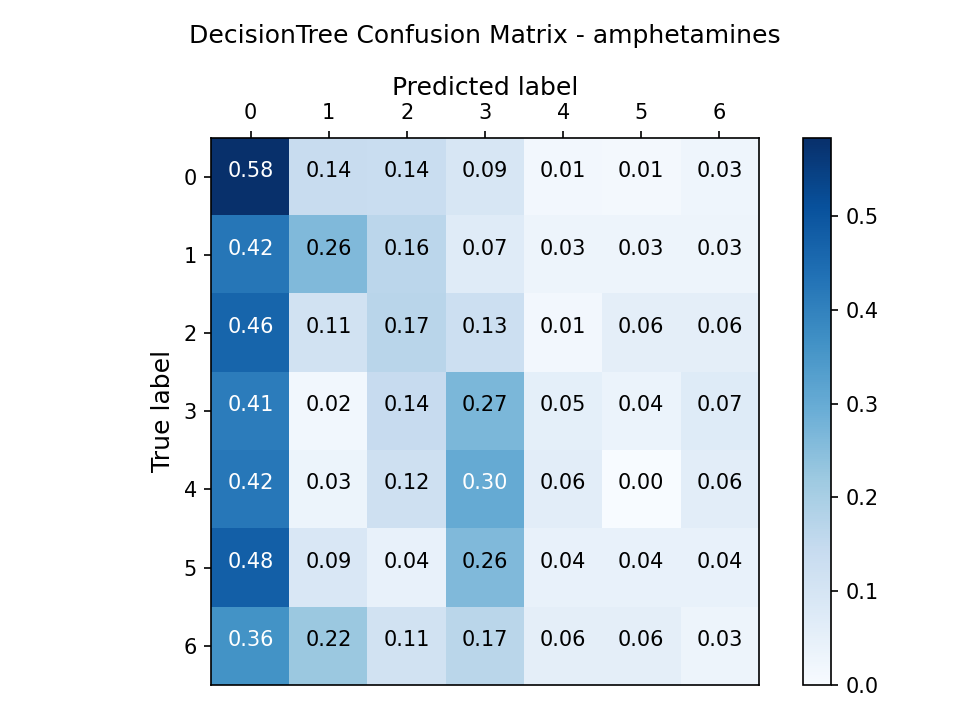
\includegraphics[width=\textwidth]{plots/m2.png}

	\end{minipage}
	\begin{minipage}[b]{0.49\textwidth}
		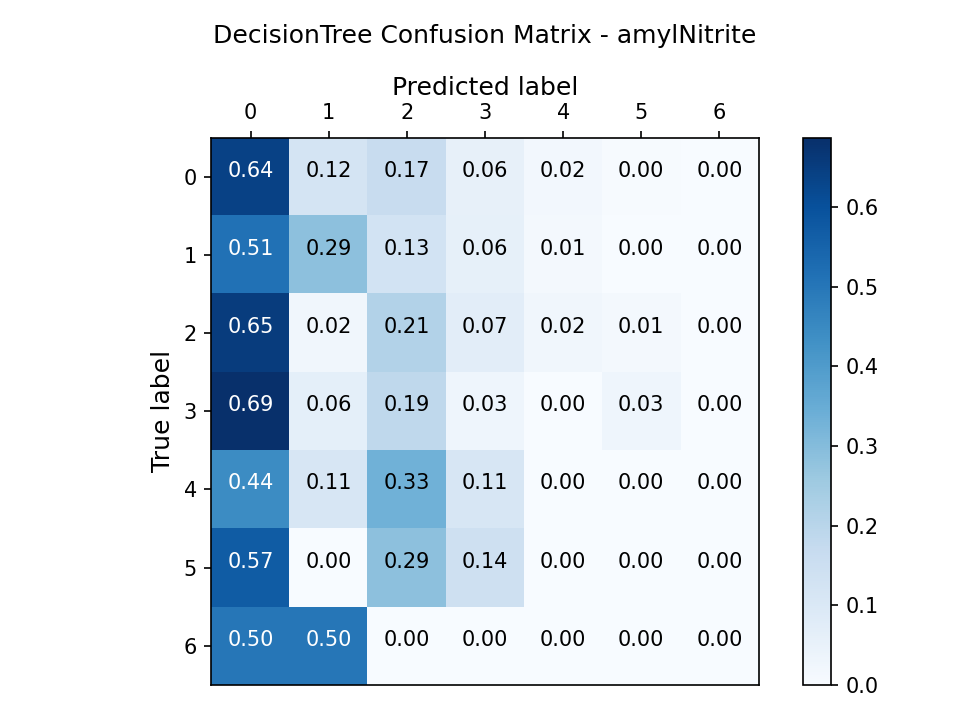
\includegraphics[width=\textwidth]{plots/m1.png}

	\end{minipage}

	\caption{Example confusion matrices for {\color{red} XXX }  }
	\label{confusion_matrices}
\end{figure}



\clearpage
\bibliography{literature.bib}{}
\bibliographystyle{unsrt}

\end{document}
